\documentclass{article}

% Language setting
\usepackage[spanish]{babel}

% Set page size and margins
\usepackage[a4paper,top=2cm,bottom=2cm,left=3cm,right=3cm,marginparwidth=1.75cm]{geometry}
\setlength\parindent{0pt}

% Useful packages
\usepackage{amsmath}
\usepackage{graphicx}
\usepackage[colorlinks=true, linkcolor=black, urlcolor=blue]{hyperref}

% Uncomment these packages if you want to use dark mode
% \usepackage{darkmode}
% \enabledarkmode


% Title and author
\title{Trabajo Autónomo 2: Red AS65100 en GNS3}
\author{Álvaro Hernández}
\date{\today}

\begin{document}

%%%%%%%%%%%%%%%%%%%%%%%%%%%%%%%%%%

\maketitle
\tableofcontents
\newpage

\section{Configurar la red de transporte: MPLS y OSPF}

La finalidad del trabajo será realizar una red AS65100 en GNS3. La  realización de esta red implicará la gestión de los routers, la configuración de protocolos de enrutamiento y el establecimiento de diversas técnicas de enrutamiento. Se configurará estos elementos en un entorno de laboratorio utilizando simuladores como GNS3 y tecnologías como MPLS. El trabajo se dividirá en varias secciones.

\subsection{configuración de la Red Core}

La primera sección será configurar la \textbf{Red Core}, que será la red principal \textbf{MPLS} a la que conectaremos las redes de los clientes. Se usarán Routers Cisco 7200 con la imagen \textbf{c7200} del aula virtual. No se está usando la máquina virtual, sino GNS3 instalado en una distribución de Linux.

\quad

Una vez importada la imagen de los routers, lo primero será añadirlos a la maqueta y configurar los Hostnames, que en nuestra red serán: \textbf{PE1, LS1, LS2, LS3, LS4, y PE2}. Tras esto, se añadirán las \textbf{IPs} mostradas en la figura inicial. Los \textbf{Text label,} no se añadirán de la misma forma que la figura del enunciado, se modificará para posteriormente acceder de forma más fácil a cada ip. Las IP de las subredes estarán por un lado, como los nombres de los routers, y por el otro los últimos 3 dígitos de la ip de la interfaz del router y a qué interfaz se encuentra conectada. Cada Loopback se indica en la zona inferior izquierda de la figura.

Tras esto, se puede empezar a configurar las \textbf{ips de las interfaces} de los routers, y las ips de cada \textbf{loopback}.
Los comandos necesarios para el cambio de Hostname y la configuración de IPs serán:

\begin{verbatim}
    Router# configure terminal
    Router(config)# hostname PE1
    PE1(config)# interface gigabitethernet x/x
    PE1(config-if)# ip address x.x.x.x y.y.y.y
    PE1(config-if)# no shutdown
    PE1(config-if)# exit
    PE1(config)# interface Loopback0
    PE1(config-if)# ip address x.x.x.x y.y.y.y
    PE1(config-if)# exit
    PE1(config)# exit
    Router# write memory
\end{verbatim}
Se adaptarán estos comandos para cada Router y para cada interfaz distinta. Es posible que existan comandos abreviados en las capturas\textsuperscript{\hyperlink{nota1}{1}}. Se explica en el apartado de notas.
Finalmente, la configuración inicial se verá de esta forma:
\begin{figure}[h]
    \centering
    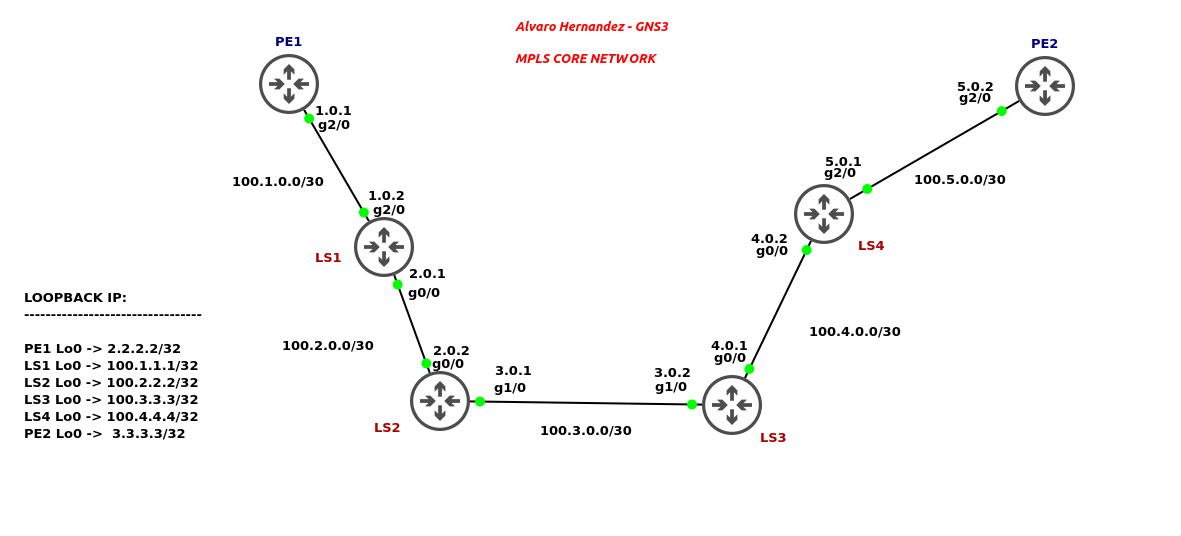
\includegraphics[width=1\textwidth]{src/primerafigura.png}
    \caption{Vista de la red Core tras la configuración inicial}
\end{figure}

\subsection{Configuración de OSPF}

La siguiente parte será configurar el protocolo de enrutamiento \textbf{OSPF} en la red Core. Se configurará OSPF con \textbf{id 1} en todos los routers de la red Core, y se establecerán las áreas \textbf{OSPF 0 para todas.} Se anunciarán tanto las interfaces de los routers como las loopback. La configuración se realizará con los siguientes comandos:

\begin{verbatim}
    Router# configure terminal
    Router(config)# router ospf 1
    Router(config-router)# network x.x.x.x y.y.y.y area 0
\end{verbatim}

Será importante añadir todas las redes de los interfaces conectadas a los routers, y las loopback. La máscara para las /30 será de 0.0.0.3 y las de /32 de 0.0.0.0. Dos ejemplos de configuración (LS1 y PE2) serán:

\begin{figure}[h]
    \centering
    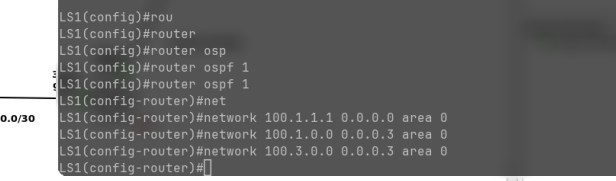
\includegraphics[width=1\textwidth]{src/ospfls1.png}
    \caption{Configuración OSPF en LS1}
\end{figure}

\begin{figure}[h]
    \centering
    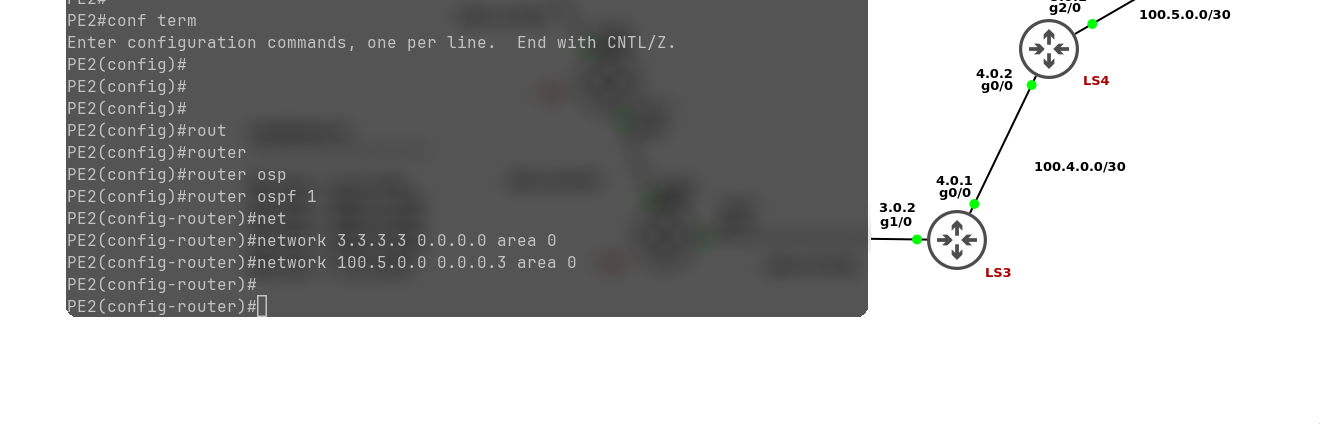
\includegraphics[width=1\textwidth]{src/pe1ospf.png}
    \caption{Configuración OSPF en PE2}
\end{figure}

Para comprobar que la configuración de OSPF es correcta, se puede usar el comando \texttt{show ip route OSPF} en los routers. Vemos en la captura que están anunciadas las demás redes. Lo que se verá en PE1 será:

\begin{figure}[h]
    \centering
    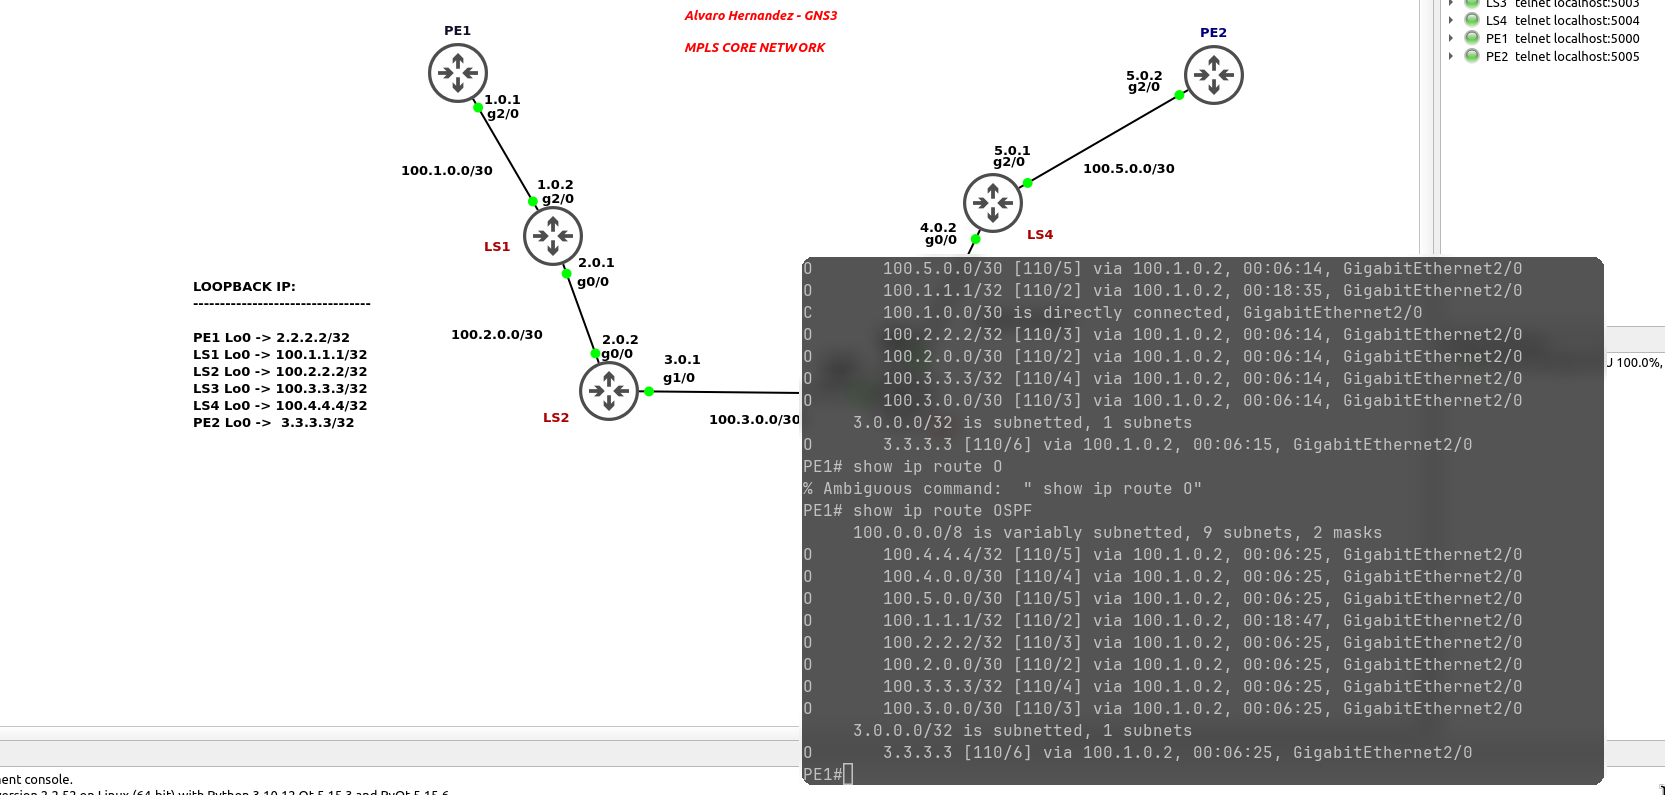
\includegraphics[width=1\textwidth]{src/segunda.png}
    \caption{Comprobación de show ip route OSPF en PE1}
\end{figure}

\newpage

\subsection{Configuración de MPLS}

Se optará por el comando \texttt{mpls ldp autoconfig} en todos los routers de la red Core. Simplemente en cada interfaz de OSPF de los routers se añadirá el comando \texttt{mpls ldp autoconfig} .
Este comando activará MPLS en todas las interfaces que tengan una dirección IP. Se comprobará que MPLS está activado con el comando \texttt{show mpls forwarding-table} en los routers. En PE1 y LS1 se verá:

\begin{figure}[h]
    \centering
    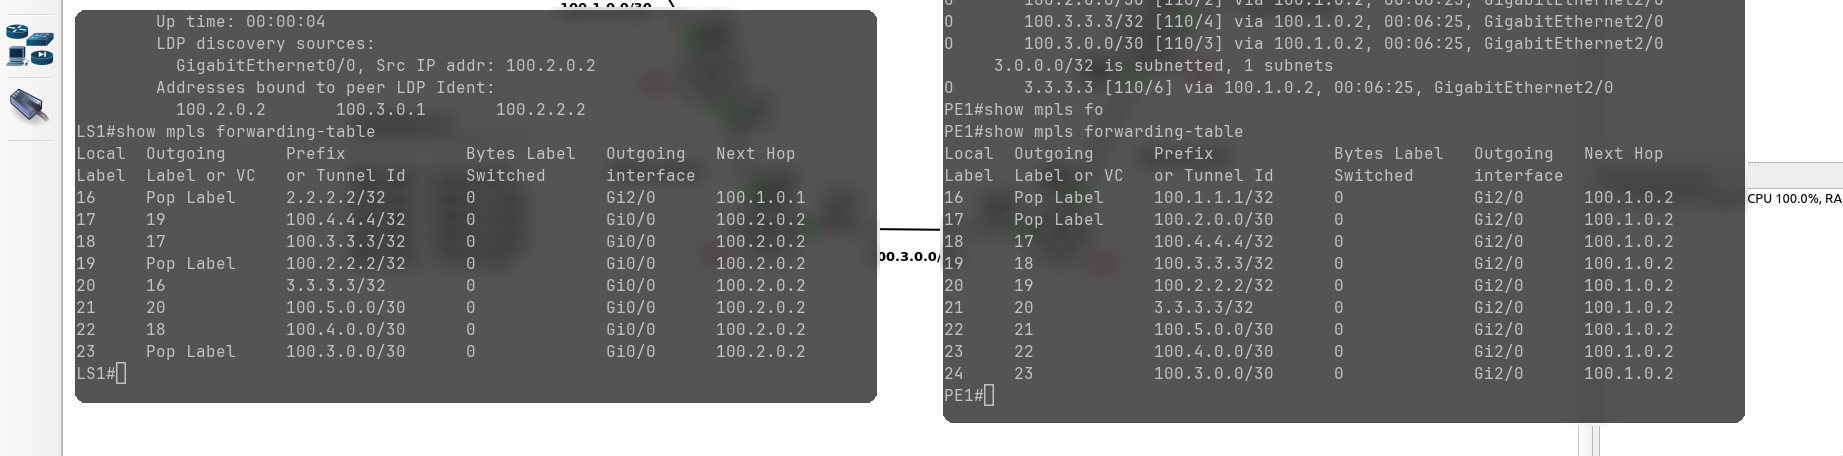
\includegraphics[width=1\textwidth]{src/showipmpls.png}
    \caption{Comprobación de show mpls interfaces en PE1 y LS1}
\end{figure}

Una vez configurado OSPF y MPLS, se puede comprobar si la conectividad. Se incluirán las capturas de los pings y traceroute requeridas en el enunciado.

\subsubsection{Comprobación de la conectividad}

Se nos pide comprobar la conectividad inicialmente indicando el ping correctamente entre \textbf{PE1 y PE2}. Se verá en la captura el ping que se realiza correctamente, seguido de un traceroute entre ambas direcciones \textbf{Loopback0}, para comprobar que el tráfico pasa por la red MPLS.
La otra comprobación será el traceroute entre las direcciones \textbf{Loopback0} de \textbf{LS3 y LS1}.

\begin{figure}[h]
    \centering
    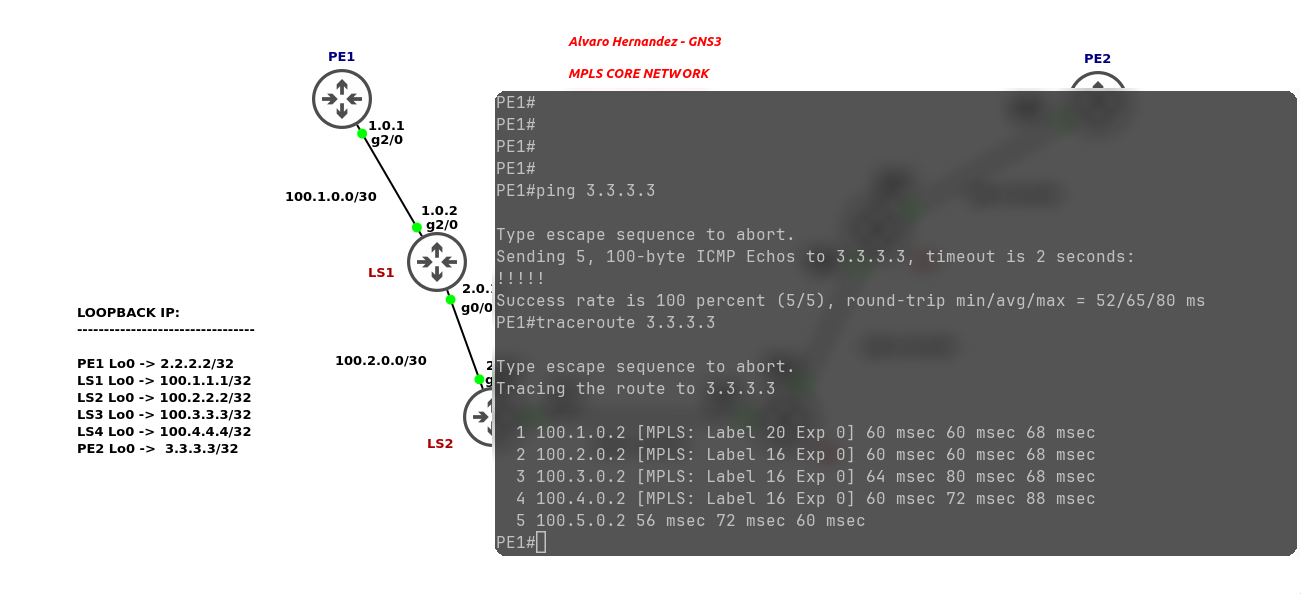
\includegraphics[width=1\textwidth]{src/pingpe1pe2.png}
    \caption{Ping entre PE1 y PE2}
\end{figure}

\begin{figure}[h]
    \centering
    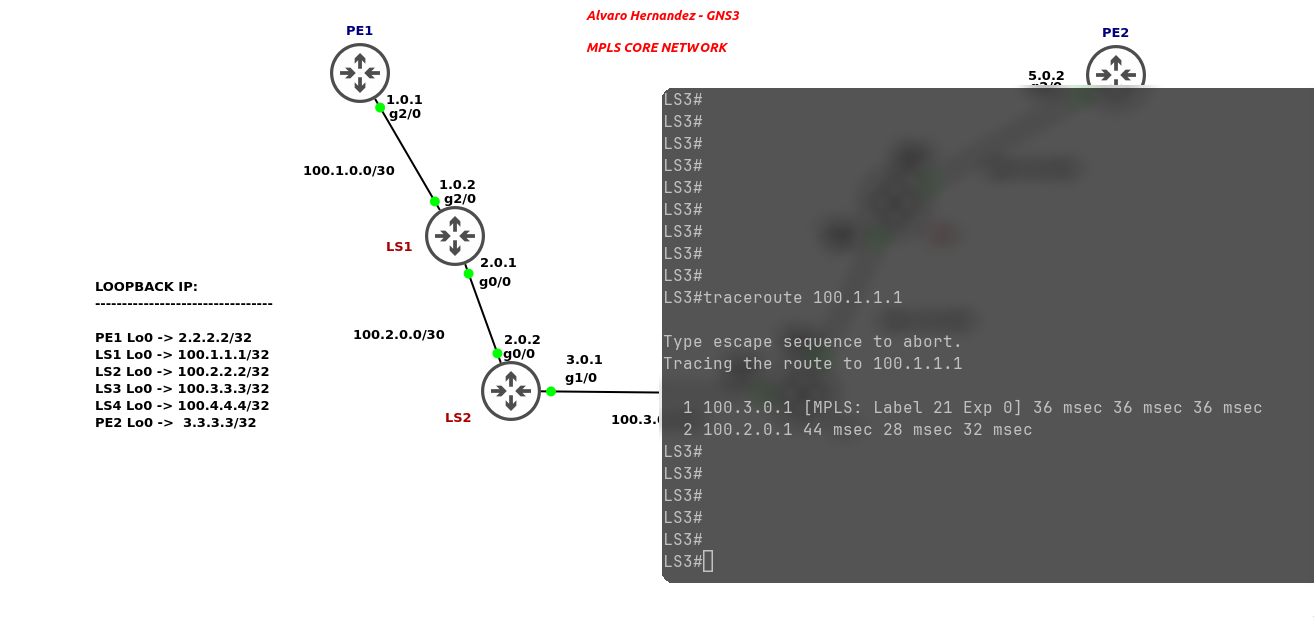
\includegraphics[width=1\textwidth]{src/tracerouteLS3.png}
    \caption{Traceroute entre LS3 y LS1}
\end{figure}


\newpage

\section{Establecimiento de la sesión iBGP}

Se establecerá una red iBGP entre los routers PE1 y PE2. Se configurará el protocolo iBGP con \textbf{id 65100} en ambos routers, y se anunciarán las direcciones de las interfaces de los routers y las loopback. Los comandos usados serán los siguientes para PE1:

\begin{verbatim}
 PE1(config)# router bgp 65100
 PE1(config-router)# neighbor [IP_LOOPBACK_PE2] update-source loopback 0
\end{verbatim}

Lo mismo para PE2, pero con la dirección de la loopback de PE1.

A continuación, se transportarán los prefijos de las redes de los clientes. Se configurará en BGP una address family. Todo esto dentro de la configuración BGP. En este caso, los comandos serán:

\begin{verbatim}
    PE1# conf term
    PE1(config)# router bgp 65100
    PE1(config-router)# address-family vpnv4
    PE1(config-router-af)# neighbor 3.3.3.3 activate
    PE1(config-router-af)# exit
    PE1(config-router)# exit
    PE1(config)# exit
    PE1# wr
\end{verbatim}

También se hará en PE2 pero con la ip del Loopback de PE1. Una vez configurados ambos, se hará la comprobación con \texttt{show bgp vpnv4 unicast all summary} en ambos routers.

\begin{figure}[h]
    \centering
    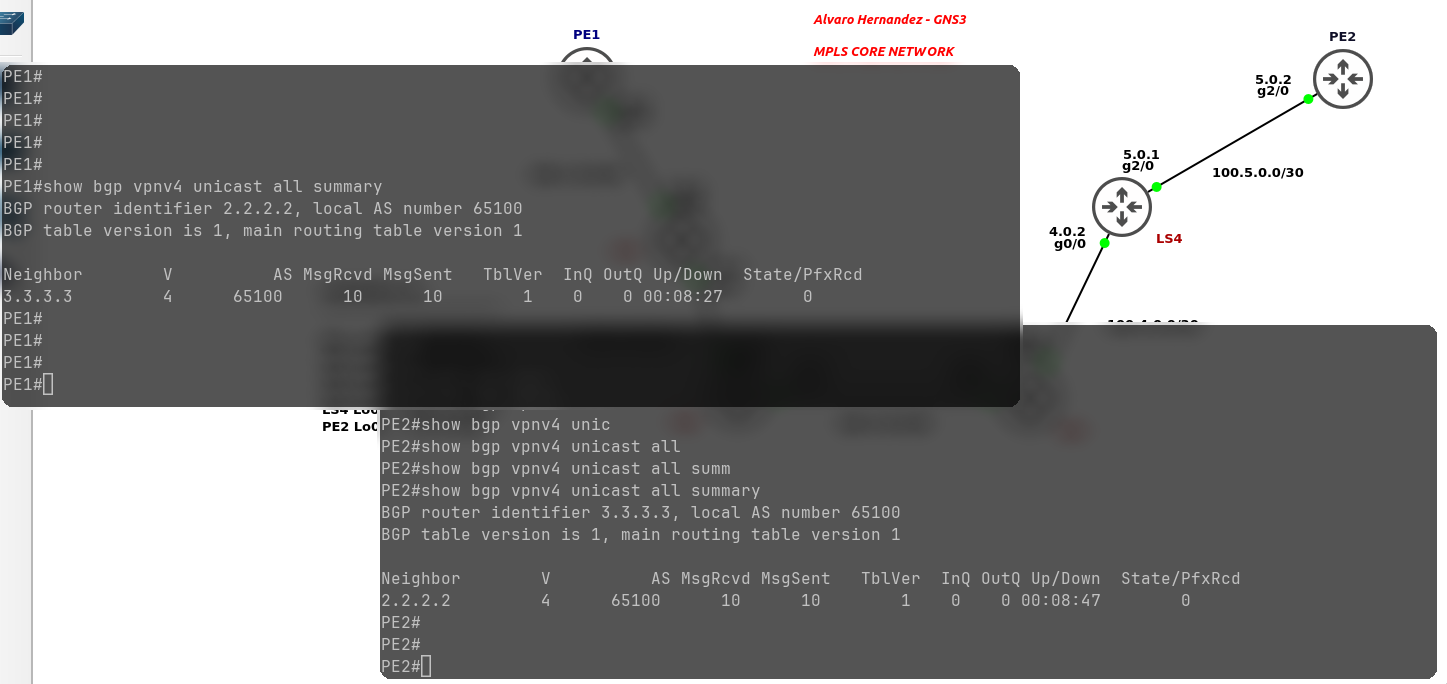
\includegraphics[width=1\textwidth]{src/vecinos.png}
    \caption{Comprobación de la sesión iBGP entre PE1 y PE2}
\end{figure}

\section{Creación de la VRF}

Se creará una VRF (Virtual Routing and Forwarding) en dos nuevos clientes que añadiremos, que serán A y B. Para empezar, recrearemos la figura inicial propuesta en el enunciado con los 4 routers de los clientes: \textbf{CE-A1, CE-A2, CE-B1 y CE-B2.}

\subsection{Configuración de los routers de los clientes}
Tras añadir los routers, que también serán c7200, los conectaremos a PE1 y PE2, y haremos la configuración inicial. Esta será de \textbf{Hostnames}, \textbf{IPs de las interfaces y delos Loopback,} y \textbf{OSPF} anunciando todas las redes conectadas y Looback que tienen cada uno. La forma de hacerlo será la misma que se ha visto hasta ahora, por lo que no se repetirá las capturas. Finalmente, la red se verá de la siguiente forma:

\begin{figure}[h]
    \centering
    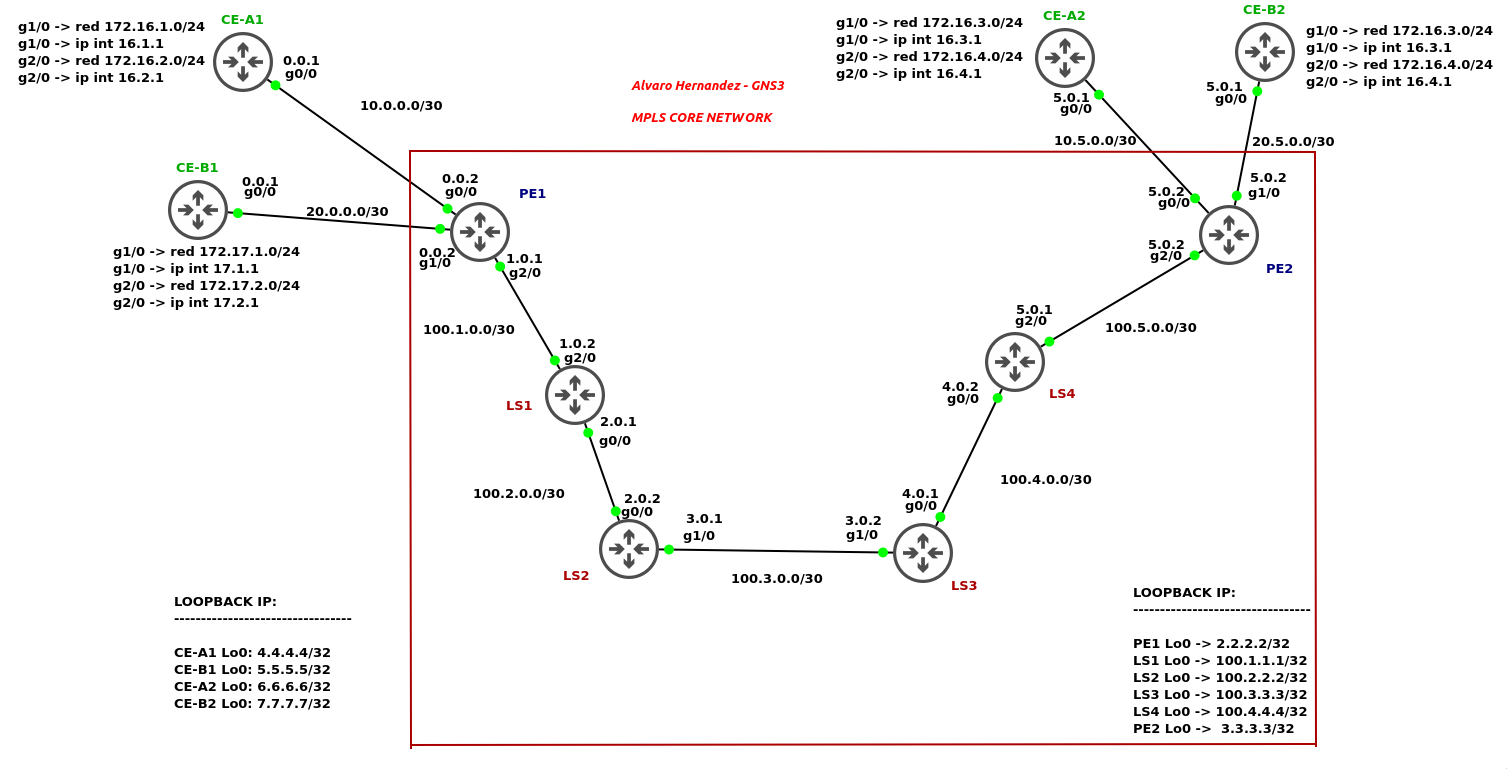
\includegraphics[width=1\textwidth]{src/ClientesNuevos.png}
    \caption{Red con los routers de los clientes}
\end{figure}

Los Text label y las líneas se han añadido en GNS3 para hacer más fácil la configuración posterior y la accesibilidad. Dentro del rectángulo, estaría nuestra red Core MPLS.

Se ha usado la ID de \textbf{OSPF} 1, y el área para el cliente A será la 2, y el del cliente B será la 4.

\subsection{VRF para los clientes A y B}

Crearemos un VRF con el nombre de \textbf{CUST-A} para el cliente A, y otro con el nombre de \textbf{CUST-B} para el cliente B. Se configurará en PE1 y PE2. Los comandos serán los siguientes:

\begin{verbatim}
    PE1# conf term
    PE1(config)# ip vrf CUST-A
    PE1(config-vrf)# rd 65100:11
    PE1(config-vrf)# route-target both 65100:11
    PE1(config-vrf)# exit
    PE1(config)# interface g0/0
    PE1(config-if)# ip vrf forwarding CUST-A
    PE1(config-if)# ip address 10.0.0.2 255.255.255.252
    PE1(config-if)# no shutdown
    PE1(config)# exit
    PE1# wr
\end{verbatim}
Estos comandos se han puesto para PE1, aunque han sido pasado a texto\textsuperscript{\hyperlink{nota2}{2}}.

De hesta forma, hemos:
\begin{itemize}
    \item Creado un VRF con el nombre de CUST-A
    \item Asignado el Route Distinguisher (RD) de 65100:11
    \item Asignado un Route Target (RT) de 65100:11
    \item Asignado la VRF a la interfaz g0/0
    \item Asignado la IP de la red que conecta PE1 a A en la interfaz g0/0
\end{itemize}

Estos comandos también se aplican con CUST-B, y luego ambos clientes se añadirán en PE2.

\subsection{Comprobación de la VRF}

Para ésto, se harán los ping que se pide, desde \textbf{PE1} a \textbf{CE-A1} y de \textbf{PE2} a \textbf{CE-B2}. Se comprobará que el ping se realiza correctamente.

\begin{figure}[h]
    \centering
    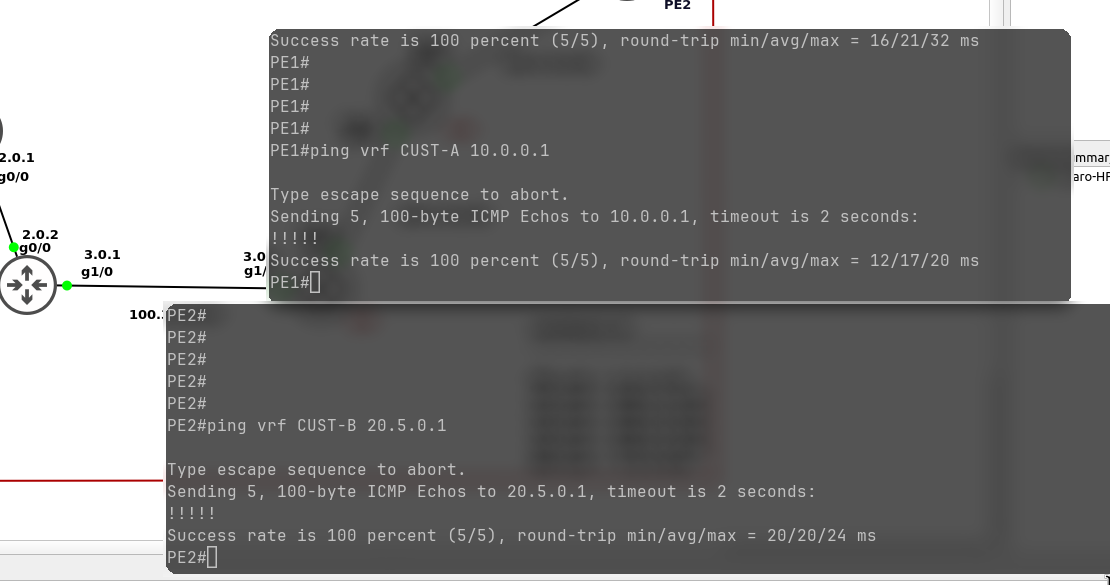
\includegraphics[width=1\textwidth]{src/pingcust.png}
    \caption{Ping a los clientes A y B}
\end{figure}

Se observa que ambos  pings se realizan correctamente, por lo que la VRF está correctamente configurada.

\section{Intercambio de rutas entre proveedor y clientes}

Actualmente, se puede hacer un png correctamente desde los routers PE a direcciones de la tabla VRF, pero no a sus Loopback. Lo añadiremos a los procesos OSPF.

Se creará para el cliente A (vrf CUST-A) un proceso OSPF con id 2 y añadiremos la red 10.0.0.0 con el wildcard 0.0.0.3, y, usaremos area 2. Haremos lo respectivo con el cliente B, la red será la 20.0.0.0 y el area 4.

\begin{verbatim}
    PE1# conf term
    PE1(config)# router ospf 2 vrf CUST-A
    PE1(config-router)# network 10.0.0.0 0.0.0.3 area 2
\end{verbatim}

\subsection{Comprobación de la conectividad}

Se hará la comprobación haciendo un ping a distintos clientes y la tabla vrf:

\begin{figure}[h]
    \centering
    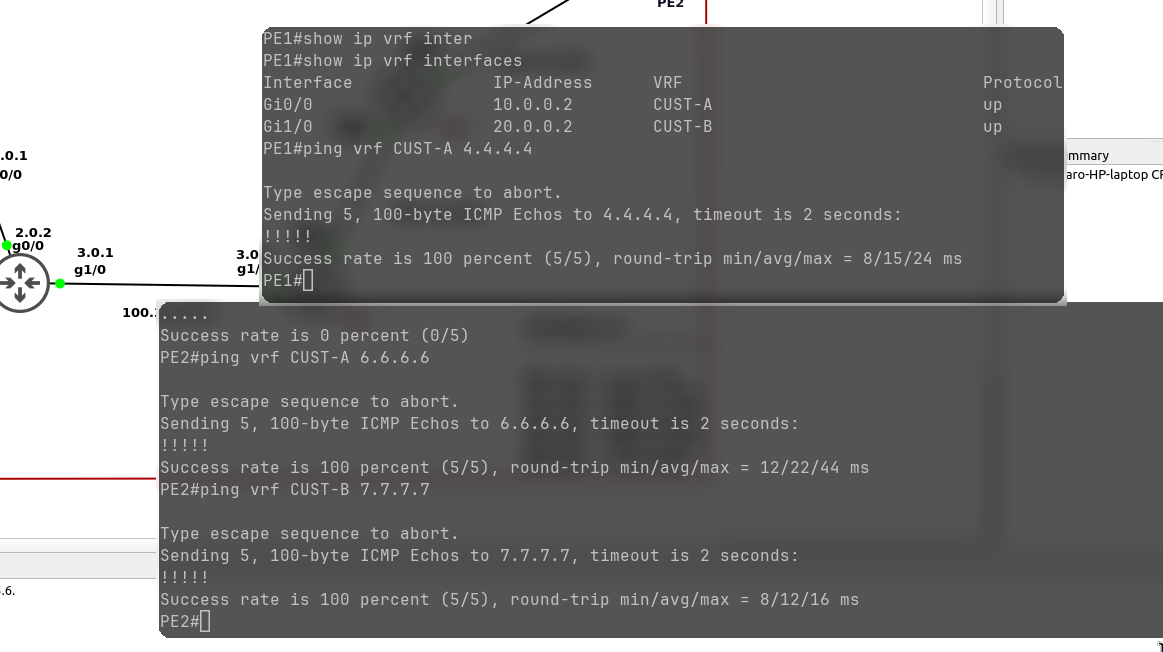
\includegraphics[width=1\textwidth]{src/custpings.png}
    \caption{Comprobación de conectividad entre clientes y routers}
\end{figure}

\section{Redistribución de rutas}
Es necesario redistribuir las rutas que se reciben de los routers CE en el proceso OSPF de la red Core. Se configurará para ambos routers PE1 y PE2.

\subsection{Comprobación inicial}

\begin{figure}[h]
    \centering
    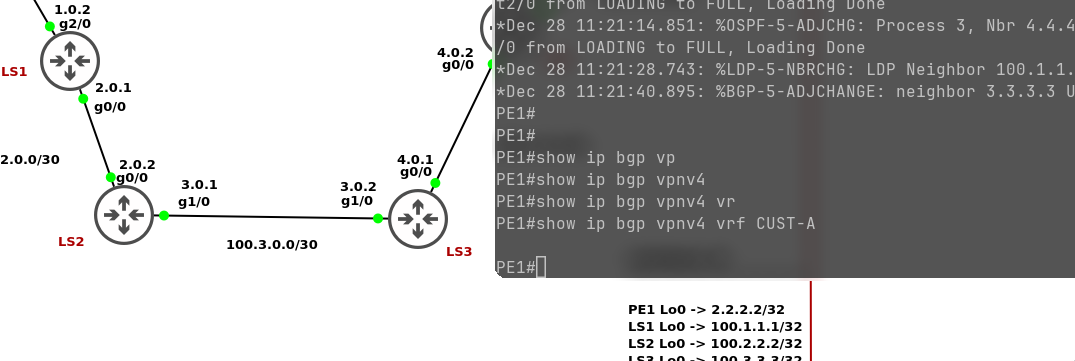
\includegraphics[width=1\textwidth]{src/ipvpn4vacia.png}
    \caption{Comprobación de la tabla OSPF vacia en PE1}
\end{figure}

Como comprobación inicial comprobamos que actualmente no hay redistribución, por lo que no hay rutas de los clientes en la tabla OSPF.

\newpage
\subsection{Configuración de la redistribución}

Para realizar la redistribución, se entrará en la configuración de nuestro sistema 65100, y se añadirá para cada id de OSPF, y la familia \textbf{ipv4} y \textbf{vrf}.

\begin{figure}[h]
    \centering
    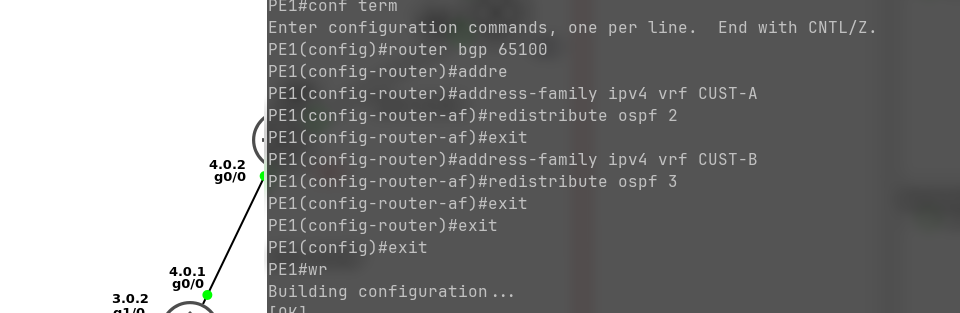
\includegraphics[width=0.9\textwidth]{src/addressfamily.png}
    \caption{Configuración de la address family en PE1}
\end{figure}

Tambien se configura en PE2.

\subsection{Comprobación de la redistribución}

Se comprobará que las rutas de los clientes se han redistribuido correctamente en . Donde ahora aparecen los vecinos correspondientes..

\begin{figure}[h]
    \centering
    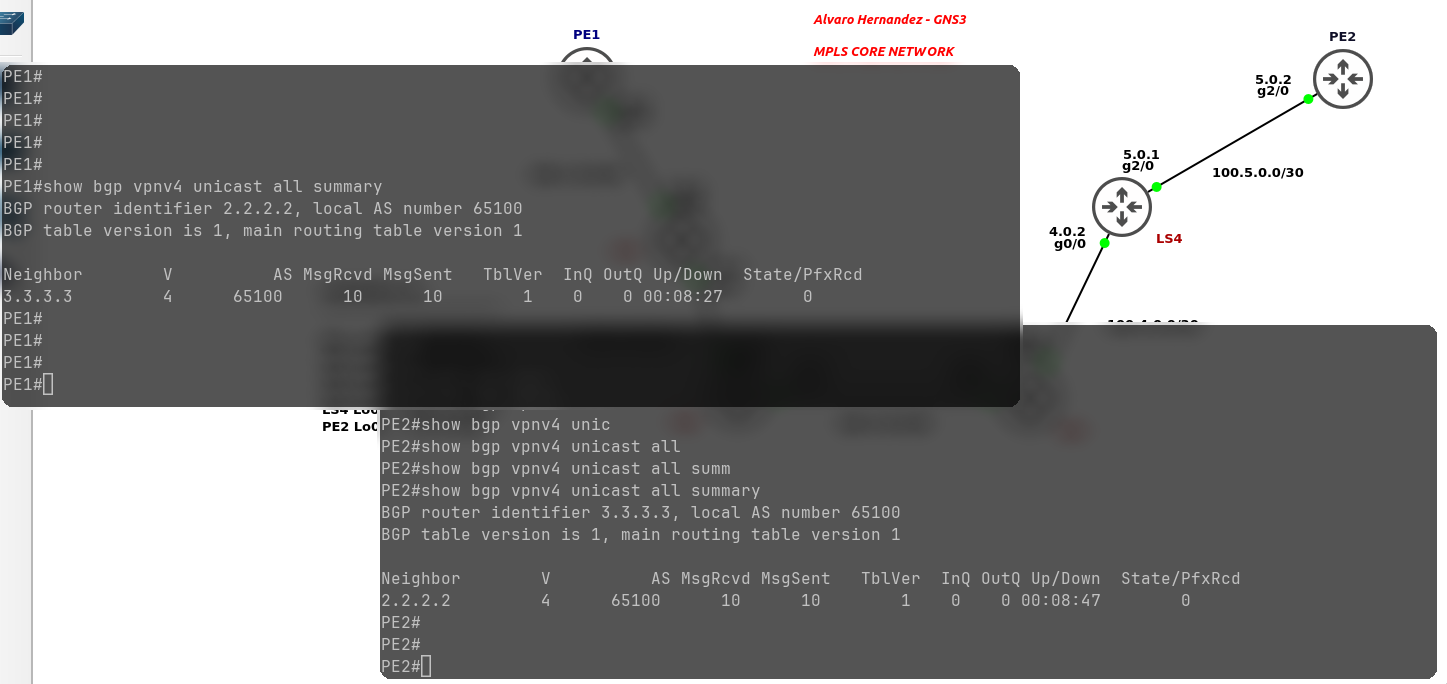
\includegraphics[width=0.9\textwidth]{src/vecinos.png}
    \caption{Comprobación de las rutas de los clientes en PE1 y PE2}
\end{figure}
\newpage

\subsection{Redistribución de BGP en OSPF}

Además de la redistribución de las rutas que se transportan con BGP en nuestra red core, es necesario también redistribuir las rutas de BGP en OSPF que usan los clientes A y B. Para ello, se hará con dos comandos para los clientes A y B, en los routers PE1 y PE2.

\begin{verbatim}
    PE1(config)# router ospf 2 vrf CUST-A
    PE1(config-router)# redistribute bgp 65100 subnets
\end{verbatim}

Se hará lo mismo para el cliente B y el router PE2, y se comprobará que las rutas se han redistribuido correctamente.

\section{Comprobacion final}

Se adjuntan las capturas correspondientes para la comprobación final de la red. Se puede apreciar que todo está correctamente configurado y que las rutas se han redistribuido correctamente. Los tres comandos correspondientes para A1 serán:

\begin{figure}[h]
    \centering
    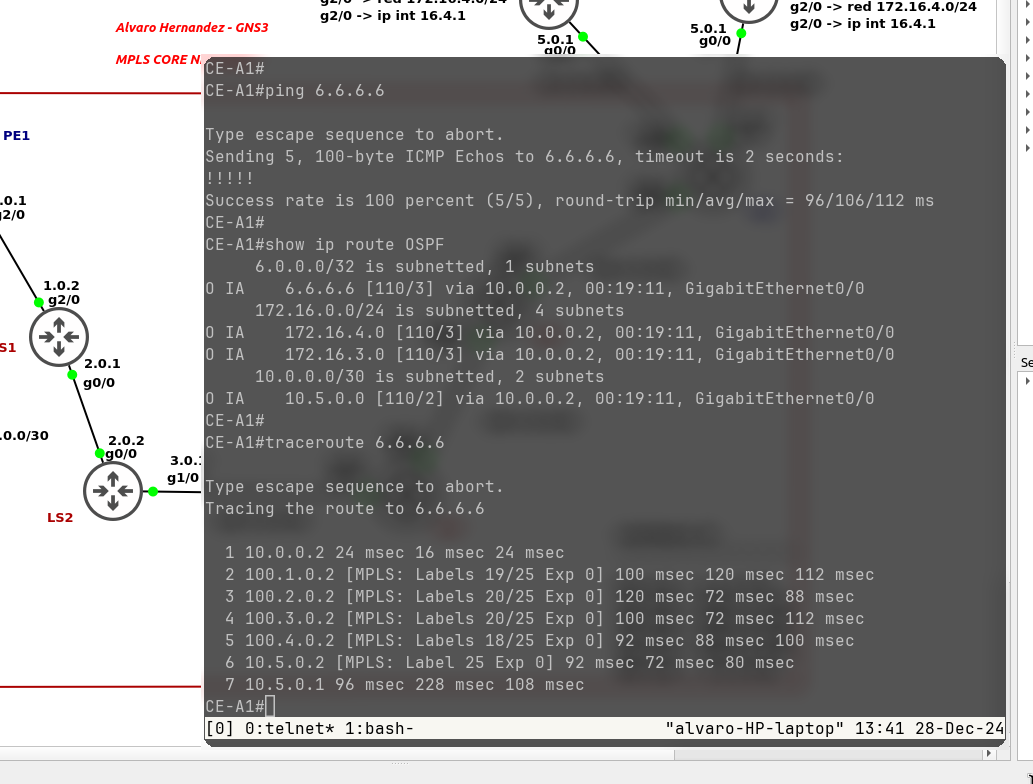
\includegraphics[width=1\textwidth]{src/comprobacion1.png}
    \caption{Comprobación final en CE-A1}
\end{figure}

Y los 3 de A2 serán:

\begin{figure}[h]
    \centering
    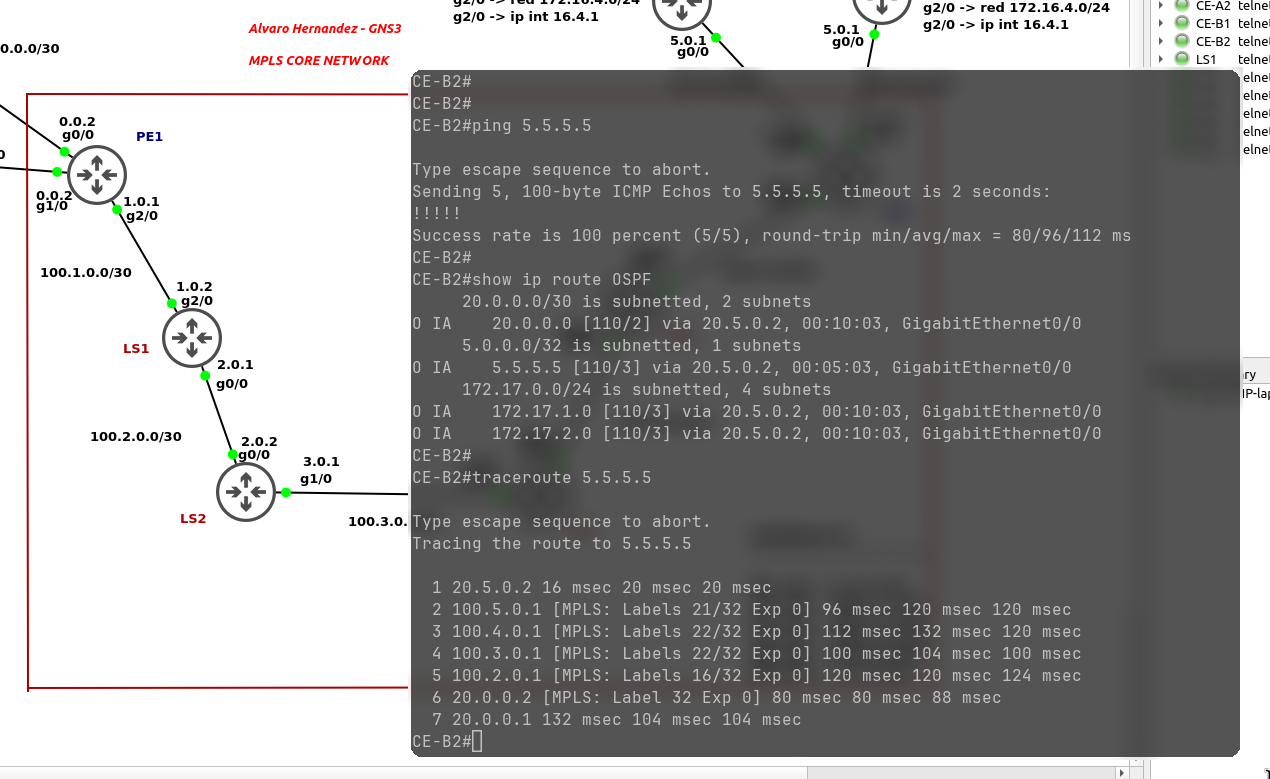
\includegraphics[width=0.9\textwidth]{src/comprobacion2.png}
    \caption{Comprobación final en CE-A2}
\end{figure}

\newpage
\section{Añadir un tercer cliente a la red MPLS}

La red MPLS está configurada correctamente para poder añadir un tercer cliente. Se añadirá un nuevo cliente, que será el cliente C, y se configurará de la misma forma que los anteriores. Se añadirá a PE1 y PE2, y se configurará OSPF y BGP para el nuevo cliente. El orden que se seguirá será el mismo que con los dispositivos anteriores. Los rouers CE-C1 y CE-C2 se añadirán a la red de la siguiente forma:

\begin{figure}[h]
    \centering
    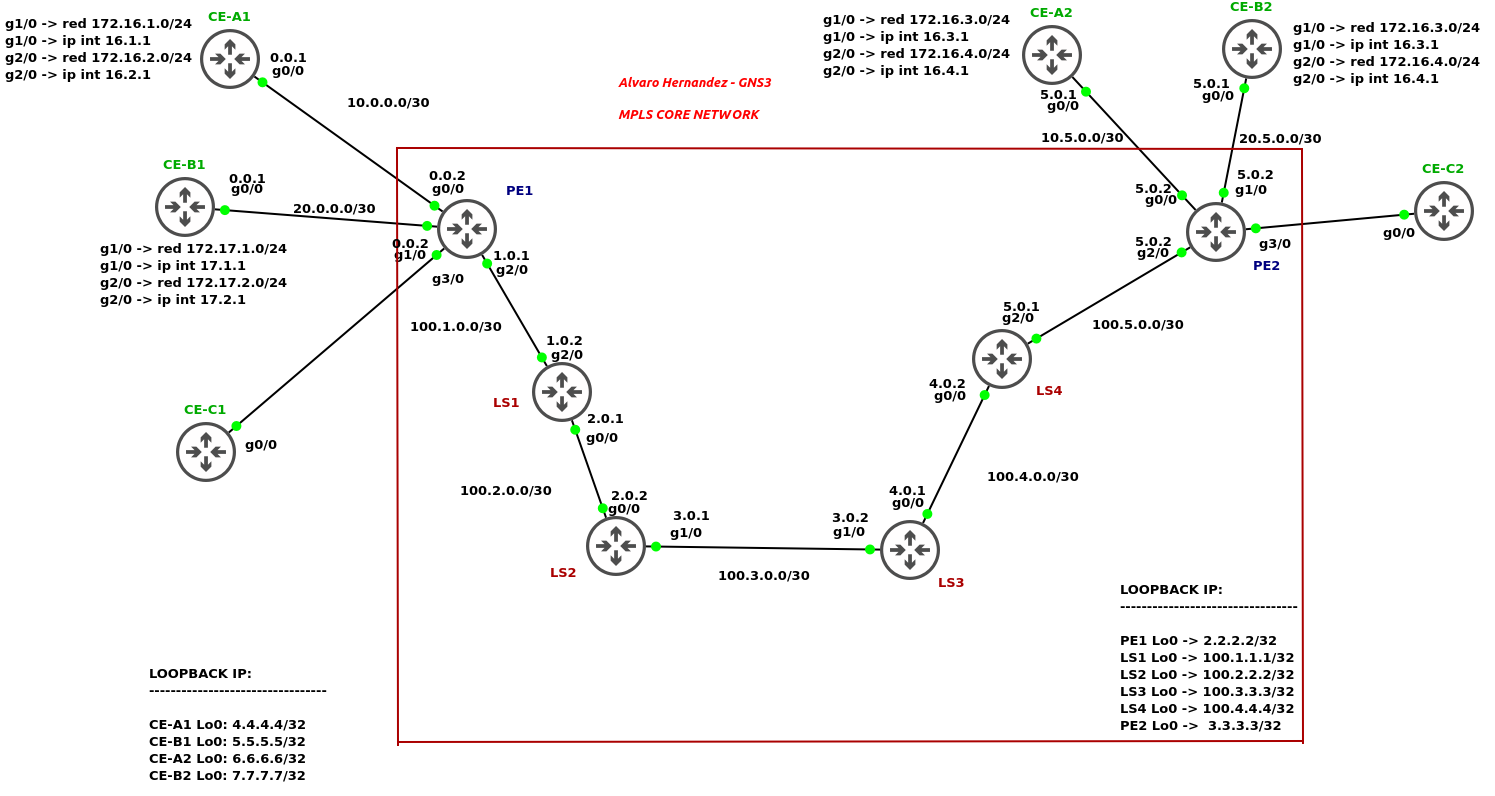
\includegraphics[width=1\textwidth]{src/red.png}
    \caption{Red con los routers de los clientes}
\end{figure}

No se ha optado por añadir los Text Labels del cliente C, ya que al ser solo un cliente se puede hacer de una forma más rápida sin necesidad de ayuda en la maqueta. Aun así, las IPs están descritas en el enunciado.
Los Loopback de los clientes C serán \textbf{8.8.8.8} para C1 y \textbf{10.10.10.10} para C2.
Para ver los datos de los clientes C, se usa la figura adjunta en el enunciado:

\begin{figure}[h]
    \centering
    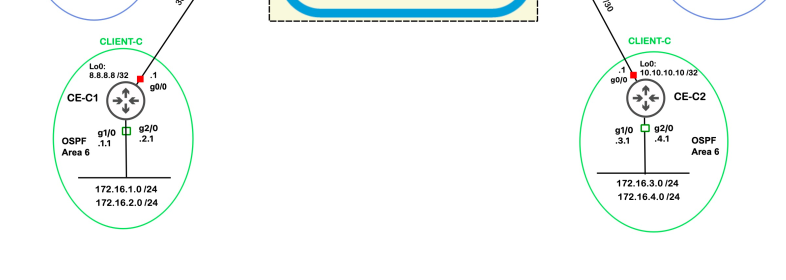
\includegraphics[width=1\textwidth]{src/ejemploip.png}
    \caption{Datos de los clientes C}
\end{figure}
\newpage
La configuración para C1 será:

\begin{verbatim}
interface Loopback0
 ip address 8.8.8.8 255.255.255.255
 no shutdown
interface GigabitEthernet0/0
 ip address 30.0.0.1 255.255.255.252
 no shutdown
interface gig1/0
 ip address 172.16.1.1 255.255.255.0
 no shutdown
interface gig2/0
 ip address 172.16.2.1 255.255.255.0
 no shutdown
exit
router ospf 1
 network 8.8.8.8 0.0.0.0 area 6
 network 30.0.0.0 0.0.0.3 area 6
 network 172.16.1.0 0.0.0.255 area 6
 network 172.16.2.0 0.0.0.255 area 6

\end{verbatim}

Esto recoge la configuración de las interfaces y la configuración de OSPF. Se hará lo mismo para C2, y se añadirá a PE1 y PE2. En PE1 y PE2 se harán las configuraciones que hemos estado haciendo hasta ahora, con las IPs de C, y se comprobará que la red se ha añadido correctamente.
Las comprobaciones finales serán:

\begin{figure}[h]
    \centering
    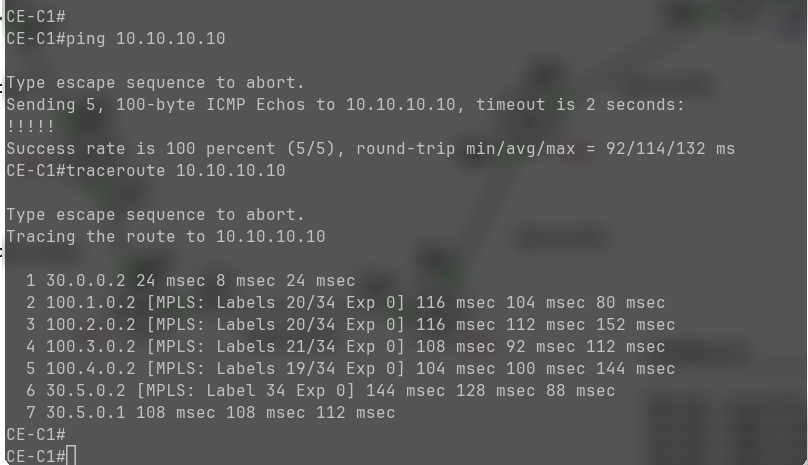
\includegraphics[width=0.7\textwidth]{src/comprobacionC1.png}
    \caption{Comprobación final CE-C1 }
\end{figure}
\begin{figure}[h]
    \centering
    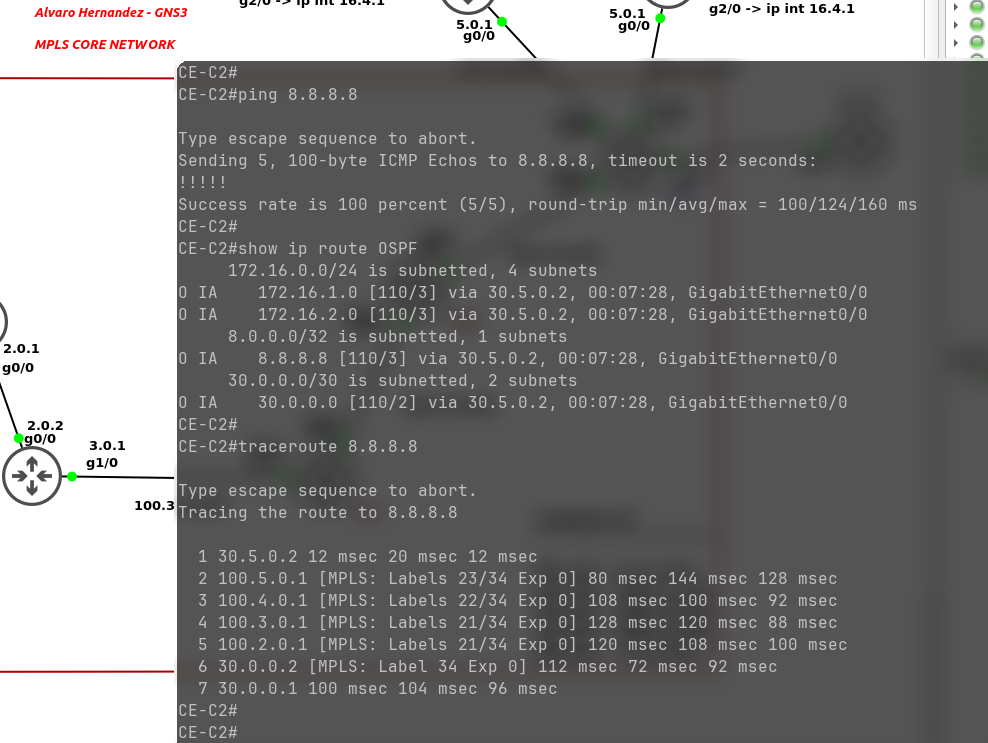
\includegraphics[width=0.9\textwidth]{src/comprobacionC2.png}
    \caption{Comprobación final pings y traceroute de CE-C2}
\end{figure}
\newpage
\begin{figure}[h]
    \centering
    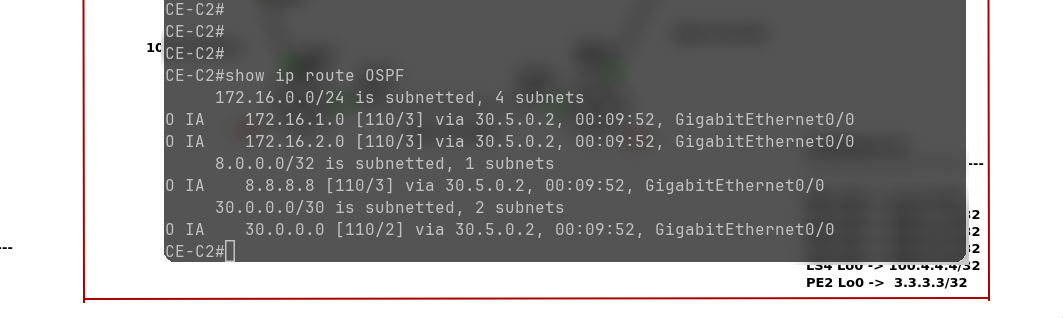
\includegraphics[width=1\textwidth]{src/iproutec2.png}
    \caption{ip route CE-C2}
\end{figure}

Con esto el tercer cliente está añadido correctamente.

\newpage
\section*{Notas sobre el trabajo}
\hypertarget{nota1}{\textsuperscript{1}} Se usarán comandos abreviados en el router que no cambian la funcionalidad del comando. Por ejemplo, \texttt{conf t} en lugar de \texttt{configure terminal}. Es posible que en las capturas aparezcan estos comandos en vez de los completos. Los más usados serán:
\begin{itemize}
    \item \texttt{conf t} o \texttt{conf term} para \texttt{configure terminal}
    \item \texttt{wr} para \texttt{write memory}
    \item \texttt{int gx/x} para \texttt{interface gigabitethernet x/x}
\end{itemize}

\hypertarget{nota2}{\textsuperscript{2}} Se han pasado los comandos a texto para que sea más fácil de leer, ya que en la captura original no estaba de forma compacta. Los comandos puestos en \texttt{este formato} se añadieron al router.

\quad

\hypertarget{nota3}{\textsuperscript{3}} La maqueta completa de GNS3 está disponible en un servidor HTTP montado gracias a un servidor virtual que nos proporciona Azure a los estudiantes de la UPCT. Estará disponible hasta iniciar el segundo cuatrimestre. La dirección es \url{https://varo6.me/maquetarba/}.
\end{document}
